\documentclass[a4paper]{article}

%% Language and font encodings
\usepackage{t1enc}
\usepackage[utf8]{inputenc}
\usepackage[magyar]{babel}

%% Sets page size and margins
\usepackage[a4paper,top=3cm,bottom=2cm,left=3cm,right=3cm,marginparwidth=1.75cm]{geometry}

%% Useful packages
\usepackage{amsmath}
\usepackage{graphicx}
\graphicspath{ {images/} }
\usepackage[colorinlistoftodos]{todonotes}
\usepackage[colorlinks=true, allcolors=blue]{hyperref}
\usepackage{listings}
\usepackage{color}
\frenchspacing

\DeclareMathOperator*{\argmax}{arg\,max}

\lstset{literate=
 {á}{{\'a}}1 {é}{{\'e}}1 {í}{{\'i}}1 {ó}{{\'o}}1 {ú}{{\'u}}1
 {Á}{{\'A}}1 {É}{{\'E}}1 {Í}{{\'I}}1 {Ó}{{\'O}}1 {Ú}{{\'U}}1
 {ö}{{\"o}}1 {ü}{{\"u}}1 {Ö}{{\"O}}1 {Ü}{{\"U}}1
 {ű}{{\H{u}}}1 {Ű}{{\H{U}}}1 {ő}{{\H{o}}}1 {Ő}{{\H{O}}}1
}

% A kódrészletek beállításai
\definecolor{codegray}{rgb}{0.5,0.5,0.5}
\lstset{xleftmargin=15pt,
        basicstyle=\scriptsize,
        numbers=left,
        numbersep=5pt,
        numberstyle=\tiny\color{codegray},
        escapechar=@,
        aboveskip=2em,
        belowskip=2em,
        belowcaptionskip=2em}

\renewcommand{\lstlistingname}{Kódrészlet}
\renewcommand{\figurename}{Ábra}


\title{Adatbányászat beadandó projekt \\  \vspace*{3pt} \large Naive Bayes m-estimate}
\author{Bagossy Attila (V8YRAZ)}

\begin{document}
\maketitle

\section{Bevezetés}

A beadandó projekt részeként egy új RapidMiner operátort készítettem, mely egy \textit{m-estimate} valószínűségi becslést alkalmazó Naiv Bayes-osztályozót biztosít a felhasználók számára. Az operátor forráskódja elérhető a következő címen:

\begin{center}
    \url{https://github.com/battila7/rapidminer-naive-bayes-m-estimate}
\end{center}

\section{A forráskód}

\subsection{Konfigurációs állományok}

Az operátor (és az azt tartalmazó plugin) megfelelő működéséhez számos konfigurációs állományra van szükség, melyek az operátor által elvárt bemenetekkel, paraméterekkel és az operátor grafikus felületen való megjelenésével kapcsolatos metaadatokat tartalmaznak. A konfigurációs állományok az \texttt{src/main/resources} mappában helyezkednek el. A továbbiakban csupán a lényegesebb állományokat ismertetem.

\subsubsection{\texttt{i18n/OperatorsDocNaiveBayesm-estimate.xml}}

Ebben az állományban adhatjuk meg az operátor nevét és azt a csoportot, amiben a felületen meg fog jelenni. Előbbi jelen esetben a \texttt{Naive Bayes (m-estimate)}, míg utóbbi a \texttt{Modeling}.

Habár ebben a fájlban megadható az operátor és a csoport neve több nyelven is, a projekt részeként csupán az angol nevek kerültek hozzáadásra.

\subsubsection{\texttt{groupsNaiveBayesm-estimate.properties}}

A különböző modelleket létrehozó operátorok a RapidMinerben általában egy zöldes színnel rendelkeznek. Annak érdekében, hogy az új operátor konzisztens megjelenéssel bírjon, ebben a fájlban ugyanezt a színt rögzítettem.

\subsubsection{\texttt{OperatorsNaiveBayesm-estimate.xml}}

A modelleket képző operátorok közös jellemzője a színen felül a villanykörtére hasonlító ikon. Az említett fájlban ezen ikon hozzárendelése történik az operátorhoz.

\subsection{Java osztályok és interfészek}

A következőkben a plugin és az operátor tényleges implementációját adó Java típusokat tekintjük át. A típusok sorrendje követi az azok között fennálló függőségeket.

\subsubsection{\texttt{battila.rapidminer.extension.PluginInitNaiveBayes}}

Minden egyes RapidMiner pluginnak tartalmaznia kell egy inicializáló osztályt, melynek metódusait a RapidMiner elinduláskor hívja meg \textit{reflection} segítéségével.

A Naiv Bayes-osztályozóhoz nincsen szükség semmilyen egyedi inicializáló kódra, emiatt a megfelelő függvények törzsei teljesen üresek.

\subsubsection{\texttt{battila.rapidminer.extension.operator.mestimate.NaiveBayesMEstimate}}

A \texttt{NaiveBayesMEstimate} osztály írja le az operátort. Ugyanezen osztály kiterjeszti az \texttt{AbstractLearner} osztályt, melyet a RapidMiner fejlesztői kifejezetten a gépi tanulást implementáló operátorok ősosztályának szántak. Az említett osztály kiterjesztésével ugyanolyan viselkedést érhetünk el, mint a beépített operátorok, azaz az operátorunk rendelkezni fog egy, az adathalmaz számára fenntartott bemeneti porttal, valamint olyan kimeneti portokkal, mint például a létrehozott modell vagy az eredeti adathalmaz. Ezen felül számos olyan kódrészletet és metódus-implementációt tartalmaz, mely az ilyen típusú operátorok esetén azonos, egyszerűsítve ezzel a fejlesztők dolgát.

A legfontosabb metódus, melyet a klienseknek (így a \texttt{NaiveBayesMEstimate} osztálynak is) implementálnia kell, a \texttt{public Model learn(ExampleSet exampleSet)}, mely egy, az adathalmazra illeszkedő modellt állít elő. Esetünkben ez a metódus egy \texttt{NaiveBayesModel} példányt fog visszaadni.

\begin{lstlisting}[language=Java, caption={A \texttt{learn} metódus implementációja.}, captionpos=b, escapechar=$]
@Override
public Model learn(ExampleSet exampleSet) throws OperatorException {
    return new NaiveBayesModel(
        exampleSet,
        getParameterAsDouble(M_PARAMETER),
        retrievePriorValues(exampleSet));
}
\end{lstlisting}


Az operátor paraméterezését a \texttt{public List<ParameterType> getParameterTypes()} függvény megvalósításával befolyásolhatjuk. Az \textit{m-estimate} valószínűségi becslés alkalmazásához két paraméterre van szükség: az $m$ értékekére valamint az egyes osztályokhoz tartozó \textit{a priori} valószínűségi értékekre.

\begin{lstlisting}[language=Java, caption={A paraméterek definiálása.}, captionpos=b, escapechar=$]
types.add(new ParameterTypeDouble(
    M_PARAMETER,
    "This parameter defines the m value used when calculating the probability.",
    Double.MIN_VALUE,
    Double.MAX_VALUE,
    DEFAULT_M_VALUE
));

types.add(new ParameterTypeList(
    PRIOR_PARAMETER,
    "Defines the a priori (estimated) probabilities of the individual classes.",
    new ParameterTypeString(
            PRIOR_CLASS_PARAMETER,
            "A possible class."
    ),
    new ParameterTypeDouble(
            PRIOR_PROBABILITY_PARAMETER,
            "The probability of the class.",
            0,
            1
    ),
    false
));
\end{lstlisting}

\subsubsection{\texttt{battila.rapidminer.extension.operator.mestimate.NaiveBayesModel}}

A Naiv Bayes-osztályozó két legfontosabb tevékenységét, azaz a tanulást és az osztályozást is a \texttt{NaiveBayesModel} valósítja meg, mely a RapidMiner beépített \texttt{PredictionModel} osztályát terjeszti ki.

A tanulási folyamat a valószínűségi becslések kiszámítását jelenti, mely közvetlenül az osztály egy példányának létrehozásakor történik meg. A becslések meghatározása attribútumonként zajlik, az attribútumokhoz rendelt \texttt{ProbabilityCalculator} objektumok segítségével. Pontosabban, a folytonos értékeket felvevő attribútumokhoz egy \texttt{GaussianProbabilityCalculator}, míg a nominális értékeket felvevő attribútumokhoz egy \texttt{NominalProbabilityCalculator} objektum kerül létrehozásra. Természetesen a különleges szereppel (\textit{role}) rendelkező attribútumok nem lesznek figyelembe véve.

\begin{lstlisting}[language=Java, caption={A valószínűségi becsléseket meghatározó \texttt{ProbabilityCalculator} objektumok létrehozása.}, captionpos=b, escapechar=$]
final Map<String, ProbabilityCalculator.Builder> calculatorBuilders = Arrays.stream(regularAttributes)
    .collect(toMap(Attribute::getName, attribute -> {
        if (attribute.isNominal()) {
            return new NominalProbabilityCalculator.Builder(attribute, m, priors);
        }
        return new GaussianProbabilityCalculator.Builder(attribute);
    }));
\end{lstlisting}

Miután a fent említett objektumok létrejöttek, következik a bemeneti adathalmaz feldolgozása. A feldolgozás során egyfelől rögzítésre kerül, hogy az egyes osztályokba hány rekord tartozik, másfelől az egyes attribútumok értékeivel frissítésre kerülnek a megfelelő \texttt{ProbabilityCalculator} objektumok is.

\begin{lstlisting}[language=Java, caption={A bemeneti adathalmaz feldolgozása.}, captionpos=b, escapechar=$]
for (Example example : trainingExampleSet) {
    countPerClass.merge(example.getValue(labelAttribute), 1, Integer::sum);

    for (Attribute attribute : regularAttributes) {
        calculatorBuilders.get(attribute.getName()).add(example);
    }
}
\end{lstlisting}

Az osztályozás a \texttt{performPrediction} metódusban történik. A metódus egy adathalmazt kap, melyet el kell látni címkékkel. A metódus ehhez egyszerűen végigfut a bemenet minden egyes rekordján, és meghatározza az adott rekordhoz tartozó címkét, valamint egy konfidencia értéket.

\begin{lstlisting}[language=Java, caption={Adathalmaz rekordjainak osztályozása.}, captionpos=b, escapechar=$]
@Override
public ExampleSet performPrediction(ExampleSet exampleSet, Attribute predictedLabel) {
    final Attribute[] regularAttributes = exampleSet.getAttributes().createRegularAttributeArray();

    for (Example example : exampleSet) {
        final Prediction prediction = predictExample(example, regularAttributes);

        example.setValue(predictedLabel, prediction.predictedClass);

        prediction.confidenceMap.forEach(example::setConfidence);
    }

    return exampleSet;
}
\end{lstlisting}

Egy rekord osztályozása a következő képlet alapján történik:

\begin{align*}
    \hat{y} = \argmax\limits_{k \in \{1, \ldots, K\}} P(C_k) \prod\limits_{i = 1}^{n}P(x_i \; | \; C_k)
\end{align*}

ahol $C_k$ a $k$-adik osztály, $P(C_k)$ az ehhez az osztályhoz tartozó \textit{a priori} valószínűség, a produktum pedig az egyes attribútumokhoz tartozó feltételes valószínűségeken fut végig. Az osztályozó azt a $C_k$ osztályt fogja választani a rekord címkéjeként, melyhez a legnagyobb valószínűség tartozik. Az ezt megvalósító forráskód a következő:

\begin{lstlisting}[language=Java, caption={Rekord osztályozása.}, captionpos=b, escapechar=$]
private Prediction predictExample(Example example, Attribute[] regularAttributes) {
    double maxProbability = Double.MIN_VALUE;
    double summedProbability = 0;
    double predictedClass = 0;

    final Map<String, Double> confidenceMap = new HashMap<>();

    for (Map.Entry<Double, Integer> clazzEntry : countPerClass.entrySet()) {
        double clazzProbability = priors.get(clazzEntry.getKey());

        for (Attribute attribute : regularAttributes) {
            clazzProbability *= Optional.ofNullable(calculators.get(attribute.getName()))
                    .map(calculator ->
                        calculator.calculateFor(example.getValue(attribute), clazzEntry.getKey()))
                    .orElse(Double.MIN_VALUE);
        }

        summedProbability += clazzProbability;

        confidenceMap.put(labelAttribute.getMapping().mapIndex(clazzEntry.getKey().intValue()), 
                            clazzProbability);

        if (clazzProbability > maxProbability) {
            maxProbability = clazzProbability;
            predictedClass = clazzEntry.getKey();
        }
    }

    final double heyCompilerThisOneIsFinal = summedProbability;
    confidenceMap.replaceAll((clazz, probability) ->
        isNaN(probability) ? 0.0 : (probability / heyCompilerThisOneIsFinal));

    return new Prediction(predictedClass, confidenceMap);
}
\end{lstlisting}

Jól látható, hogy a kód egy maximumkereséső ciklus köré szerveződik, amely végigfut a lehetséges osztályokon. A legnagyobb valószínűséget a \texttt{maxProbability}, a kiválasztott osztályt pedig a \texttt{predictedClass} változók tartalmazzák. Egy adott osztályhoz tartozó valószínűség kiszámítása a következő módon zajlik. Először hozzárendeljük a \texttt{clazzProbability} változóhoz az osztály \textit{a priori} valószínűségét. Ezután sorra szorzunk az attribútumokhoz tartozó feltételes valószínűségekkel. Amennyiben az így kapott érték nagyobb, mint az eddigi maximális valószínűség, akkor módosítjuk a maximális értéket és a kiválasztott osztályt.
A címke meghatározásán túl, e metódusban konfidencia értékeket is kiszámítunk, melyek a \texttt{confidenceMap} változóban kerülnek tárolásra; minden osztályhoz egy valós érték. 
A metódus visszatérési értéke egy, a kiválasztott osztályt és a konfidencia értékeket tartalmazó \texttt{Map}-et magában foglaló \texttt{Prediction} objektum lesz.

\subsubsection{\texttt{battila.rapidminer.extension.operator.mestimate.NominalProbabilityCalculator}}

A \texttt{NominalProbabilityCalculator} osztály számítja ki nominális attribútumokra a valószínűségi becsléseket. Egy adott attribútumértékre a következő módon határozza meg a becslést:

\begin{align*}
P(x_i \; | \; C) = \frac{N_{ic} + mp}{N_{c} + m},
\end{align*}

ahol $N_{ic}$ a $C$ osztályba tartozó, az adott attribútumértékkel rendelkező rekordok száma, $N_{c}$ az összes $C$ osztálybeli rekord száma, $m$ egy felhasználó által megadott érték, $p$ pedig a $C$ osztály \textit{a priori} valószínűsége.

Implementációt tekintve, a \texttt{NominalProbabilityCalculator} osztály \texttt{calculateFor} metódusa felelős a valószínűség kiszámításáért. A metódus kap egy attribútumértéket, valamint egy osztályt, és visszaadja az ezekhez számolt valószínűséget. Ehhez a tanulási folyamat során meghatározott értékeket használja fel, azaz azt, hogy egy adott attribútumértékhez hány adott osztálybeli rekord tartozott, valamint, hogy attribútumoktól függetlenül, hány adott osztálybeli előfordulás volt.

\pagebreak

\begin{lstlisting}[language=Java, caption={Nominális attribútum feltételes valószínűségének kiszámítása.}, captionpos=b, escapechar=$]
@Override
public double calculateFor(double attributeValue, double clazz) {
    final int count = valueCountPerClass.get(attributeValue).get(clazz);

    final double numerator = (double)count + m * priors.get(clazz);

    return numerator / (countPerClass.get(clazz).doubleValue() + m);
}
\end{lstlisting}

\subsubsection{battila.rapidminer.extension.operator.mestimate.GaussianProbabilityCalculator}

Folytonos attribútumokhoz tartozó valószínűségi becsléseket a \texttt{GaussianProbabilityCalculator} osztály képes számolni. Ahogy az osztály neve is mutatja, feltesszük, hogy az attribútum normális eloszlású, majd pedig a bementi adathalmaz alapján megbecsüljük az eloszlás paramétereit.

Amikor számítanunk kell egy adott feltételes valószínűséget, akkor vesszük az adott osztályhoz tartozó paramétereket, és azok alapján becsüljük az attribútumértékhez és az osztályhoz tartozó feltételes valószínűséget. A paramétereket a \texttt{distributionPropertyMap} tartalmazza, melyet a tanulási fázis során töltünk fel értékekkel.

\begin{lstlisting}[language=Java, caption={Nominális attribútum feltételes valószínűségének kiszámítása.}, captionpos=b, escapechar=$]
@Override
public double calculateFor(double attributeValue, double clazz) {
    final DistributionProperties props = distributionPropertyMap.get(clazz);

    final double pow = -(Math.pow(attributeValue - props.mean, 2) / (2 * props.variance));

    final double rat = 1.0 / Math.sqrt(2 * Math.PI * props.variance);

    return rat * Math.exp(pow);
}
\end{lstlisting}

\section{Az operátor használata}
\subsection{Az operátor telepítése}
Az operátor telepítése előtt győződjünk meg arról, hogy a RapidMiner valamely verziója, valamint a Java Development Kit (legalább 8-as verziójú) telepítve van a számítógépünkre. Az operátor kódját tartalmazó repository klónozásához gitre is szükség van.

A telepítéshez, a repository klónozását követően, adjuk ki a következő parancsot annak gyökérkönyvtárában:

\begin{lstlisting}[language=bash, caption={Az operátor telepítése.}, captionpos=b, escapechar=$]
./gradlew installExtension
\end{lstlisting}

Ha a telepítés sikeres volt, akkor a RapidMiner elindítását követően, az \textit{Extension} menüpont \textit{About Installed Extensions} almenüjében meg fog jelenni egy \textit{About Naive Bayes m-estimate Extension} menüpont.

\pagebreak

\subsection{Titanic}

Nézzük meg az operátor használatát a Titanic adathalmazon! Ehhez az 1. ábrán látható folyamatot állítottam össze.

\begin{figure}[h]
    \centering
    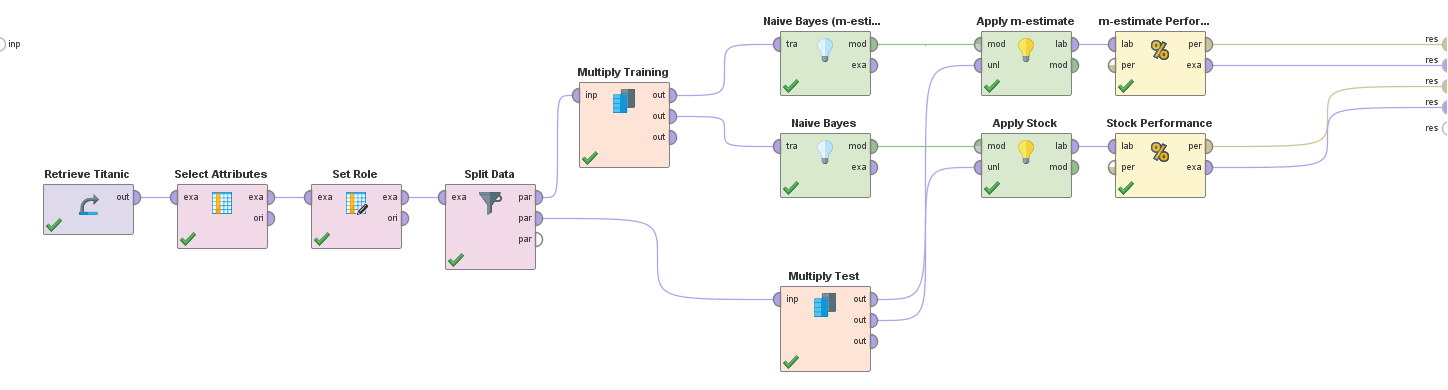
\includegraphics[width=16cm]{process}
    \caption{A Titanic adathalmaz címkézése.}
\end{figure}

A folyamat részeként összehasonlításra kerül a beépített Naiv Bayes-osztályozó, és a beadandó projekt részeként elkészült, \textit{m-estimate} módszert alkalmazó osztályozó performanciája.

\subsubsection{Select Attributes}

Az adathalmaz beolvasását követően eldobjuk azokat az attribútumokat, melyek nem lényegesek az osztályozás szempontjából. Ezek a következők:

\begin{itemize}
    \item Cabin
    \item Name
    \item TicketNumber
\end{itemize}

\subsubsection{Set Role}

A következő lépés a \textit{Survived} attribútum felruházása a \textit{Label} szerepkörrel. Ez teszi lehetővé, hogy később kiértékelhessük az osztályozók teljesítményét. Annak következtében, hogy a \textit{Survived} attribútum ilyen speciális szereppel rendelkezik, sem a tanítás, sem az osztályozás során nem lesz számításba véve, nem számít többé reguláris attribútumnak (\textit{regular attribute}.

\subsubsection{Split Data}

Az adathalmazt $7:3$ arányban felosztjuk tanító halmazra és teszt halmazra. Előbbi segítségével készítjük el a modelleket, utóbbin pedig azok teljesítményét fogjuk mérni.

\subsubsection{Naive Bayes m-estimate}

A projekt részeként elkészített operátornak két paramétere van: az $m$ érték és az \textit{a priori} valószínűségek (2. ábra).

\begin{figure}[h]
    \centering
    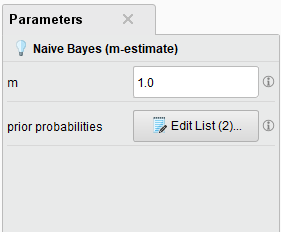
\includegraphics[width=5cm]{parameters}
    \caption{A \textit{Naive Bayes m-estimate} operátor paraméterei.}
\end{figure}

Az egyes osztályokhoz tartozó \textit{a priori} valószínűségeket egy külön párbeszédablakon állíthatjuk be (3. ábra).

\begin{figure}[h]
    \centering
    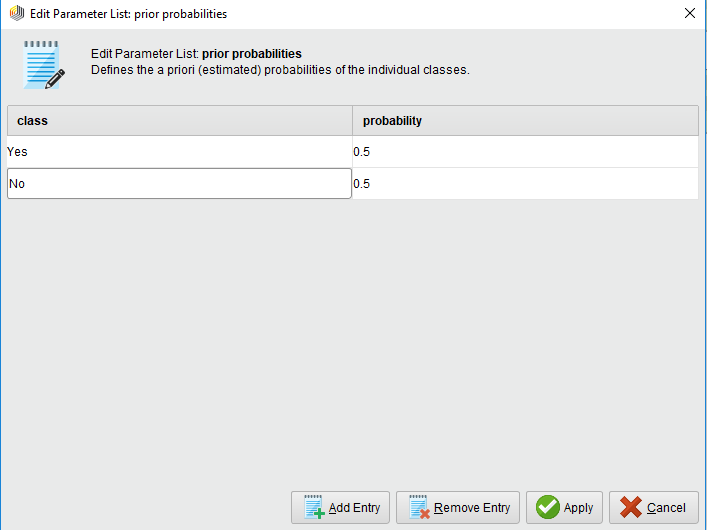
\includegraphics[width=10cm]{priors}
    \caption{Az \textit{a priori} valószínűségek beállítása.}
\end{figure}

\subsubsection{Apply m-estimate / Apply Stock}

A tanítás után következhet a modelleket tesztelése korábban nem látott adatokon. Az \textit{Apply m-estimate} operátor az \textit{m-estimate} módszert alkalmazó modellt használja, míg az \textit{Apply Stock} operátor a beépített osztályozó által előállított modellt.

\subsubsection{m-estimate Performance / Stock Performance}

A folyamat utolsó fázisa a modellek teljesítményének kiértékelése. A folyamat kimenetét az így kapott metrikák, valamint a felcímkézett adathalmazok fogják alkotni. Az eredeti operátor által adott modell teljesítménye a 4. ábrán, az \textit{m-estimate} modell teljesítménye az 5. ábrán látható.

\begin{figure}[h]
    \centering
    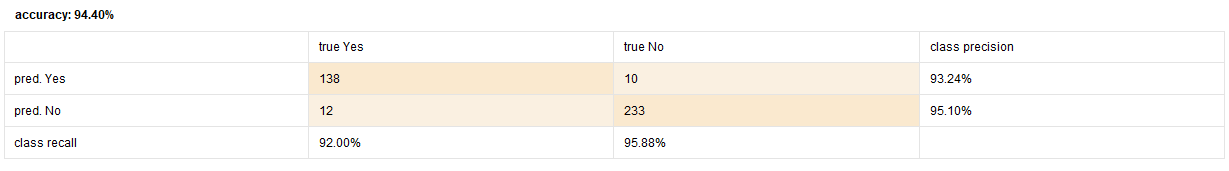
\includegraphics[width=15cm]{stock_performance}
    \caption{A beépített Naiv Bayes-osztályozó által előállított modell performanciája.}
\end{figure}

\begin{figure}[h]
    \centering
    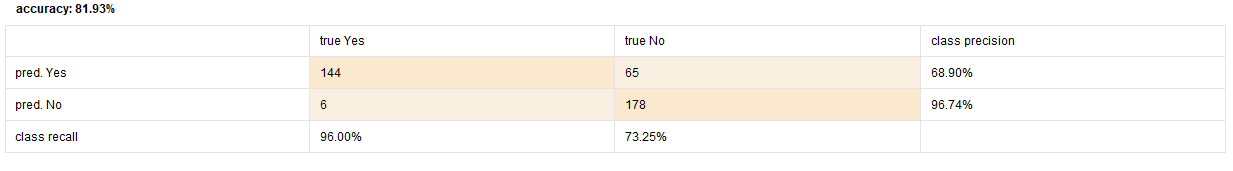
\includegraphics[width=15cm]{m_estimate_performance}
    \caption{Az \textit{m-estimate} módszert alkalmazó modell performanciája.}
\end{figure}

Leolvasható, hogy az \textit{m-estimate} módszert alkalmazó modell pontossága (\textit{accuracy}) alulmarad a beépített osztályozó pontosságához képest. Előbbi ugyanis túl sok, valójában \textit{No} címkével rendelkező rekordot sorol a \textit{Yes} osztályba. Ezen egyrészt az $m$ érték és az \textit{a priori} valószínűségek módosításával javíthatunk. Másrészt, a két operátor közötti kisebb implementációs különbségek (például a hiányzó értékek kezelésének módja) is állhatnak az eltérés mögött.

\end{document}
